% 鈴木研究室 卒業論文研究業績テンプレート
% Version: 1.1
% Last Update: 2011/12/31 by Hidekazu Suzuki
% Contact to: hsuzuki@meijo-u.ac.jp
% Character code: UTF-8

% === 学術論文(ここから)=============================
% 無ければ削除
\section*{学術論文(査読あり)}
\begin{enumerate}
\item 後藤裕司,\underline{鈴木秀和},渡邊 晃:NATをまたがる閉域通信グループの提案と評価,
情報処理学会論文誌,Vol.~52, No.~9, pp.\ 2866--2875, Sep. 2011.
\end{enumerate}
% === 学術論文(ここまで)=============================


% === 国際会議(ここから)=============================
% 無ければ削除
\section*{国際会議(査読あり)}
\begin{enumerate}
\item D. Kato, H. Yamagishi, \underline{H. Suzuki}, E. Konaka and A. Watanabe: 
Proposal of a Remote Watching System Utilizing a Smartphone and Sensors,
{\em Proc. of the 11th IEEE International Symposium on Communications and Information Technologies (ISCIT 2011)},
pp.\ 36--41, Hangzhou, China, Oct. 2011.

\item H. Yamagishi, D. Kato, K. Teshima, \underline{H. Suzuki}, O. Yamamoto and A. Watanabe: 
Proposal and Implementation of a System to Remotely Watch the Health Conditions of Elderly Persons,
{\em Proc. of the 11th IEEE International Symposium on Communications and Information Technologies (ISCIT 2011)},
pp.\ 42--47, Hangzhou, China, Oct. 2011.

\item T. Kuboshiki, \underline{H. Suzuki} and A. Watanabe: 
Proposal on the Concealment of the Network Topology in IPv6,
{\em Proc. of the 11th IEEE International Symposium on Communications and Information Technologies (ISCIT 2011)},
pp.\ 53--57, Hangzhou, China, Oct. 2011.
\end{enumerate}
% === 国際会議(ここまで)=============================


% === 査読あり国内会議(ここから)=============================
% ・DICOMOなど
% 無ければ削除
\section*{国内会議(査読あり)}
\begin{enumerate}
\item 久保敷透,\underline{鈴木秀和},渡邊 晃:IPv6 におけるネットワーク構成隠蔽の提案,
マルチメディア,分散,協調とモバイル(DICOMO2011)シンポジウム論文集,Vol.~2011,No.~1,pp.\ 323--328,Jul. 2011.

\item 鈴木健太,\underline{鈴木秀和},渡邊 晃:リモートアクセス方式GSRAの性能評価,
マルチメディア,分散,協調とモバイル(DICOMO2011)シンポジウム論文集,Vol.~2011,No.~1,pp.\ 336--343,Jul. 2011.

\item 山岸弘幸,加藤大智,手嶋一訓,\underline{鈴木秀和},山本修身,渡邊 晃:高齢者を遠隔地から見守るシステムの提案と実装,
マルチメディア,分散,協調とモバイル(DICOMO2011)シンポジウム論文集,Vol.~2011,No.~1,pp.\ 684--690,Jul. 2011.

\item 加藤大智,山岸弘幸,\underline{鈴木秀和},小中英嗣,渡邊 晃:スマートフォンとセンサを活用したリモート 見守りシステムの提案,
マルチメディア,分散,協調とモバイル(DICOMO2011)シンポジウム論文集,Vol.~2011,No.~1,pp.\ 691--696,Jul. 2011.

\item 福山陽祐,\underline{鈴木秀和},渡邊 晃:IPv4 移動体通信において携帯電話網と無線LAN間をシームレスに移動する方式の提案,
マルチメディア,分散,協調とモバイル(DICOMO2011)シンポジウム論文集,Vol.~2011,No.~1,pp.\ 1115--1120,Jul. 2011.

\item 西尾拓也, 内藤克浩, 水谷智大, \underline{鈴木秀和}, 渡邊 晃, 森香津夫, 小林英雄:NTMobileにおける端末アドレスの移動管理と実装,
マルチメディア,分散,協調とモバイル(DICOMO2011)シンポジウム論文集,Vol.~2011,No.~1,pp.\ 1139--1145,Jul. 2011.

\item \underline{鈴木秀和},水谷智大,西尾拓也,内藤克浩,渡邊 晃:NTMobileにおける相互接続性の確立手法と実装,
マルチメディア,分散,協調とモバイル(DICOMO2011)シンポジウム論文集,Vol.~2011,No.~1,pp.\ 1339--1348,Jul. 2011.

\item 内藤克浩,西尾拓也,水谷智大,\underline{鈴木秀和},渡邊 晃,森香津夫,小林英雄:NTMobileにおける移動透過性の実現と実装,
マルチメディア,分散,協調とモバイル(DICOMO2011)シンポジウム論文集,Vol.~2011,No.~1,pp.\ 1349--1359,Jul. 2011.
\end{enumerate}
% === 査読あり国内会議(ここまで)=============================


% === 査読無し国内会議(ここから)=============================
% ・東海支部連合大会,全国大会,研究会など
\section*{国内会議(査読なし)}
\begin{enumerate}
\item 上醉尾一真,\underline{鈴木秀和},内藤克浩,渡邊 晃:IPv6ネットワークにおけるNTMobileの検討,
情報処理学会研究報告,Vol.~2011-MBL-59, No.~9, pp.\ 1--7, Sep. 2011.

\item 金丸幸弘,\underline{鈴木秀和}:無線センサネットワークの可視化に関する検討,
平成23年度電気関係学会東海支部連合大会論文集,Vol.~2011,講演番号B2-7, Sep. 2011.

\item 畠 基成,\underline{鈴木秀和}:SNMPを用いたメッシュ型無線センサネットワーク管理手法の検討,
平成23年度電気関係学会東海支部連合大会論文集,Vol.~2011,講演番号B2-8, Sep. 2011.

\item 松尾辰也,\underline{鈴木秀和},旭 健作,渡邊 晃:プライベートアドレスを持つ無線メッシュネットワークとインターネットの接続方法,
平成23年度電気関係学会東海支部連合大会論文集,Vol.~2011,講演番号B4-5, Sep. 2011.

\item 横山和希,\underline{鈴木秀和},松本幸正:ZigBeeネットワークを用いたバスロケーションシステムの提案,
平成23年度電気関係学会東海支部連合大会論文集,Vol.~2011,講演番号B4-5, Sep. 2011.

\item 五島秀典,\underline{鈴木秀和},渡邊 晃:秘密情報を保持しないクライアントを用いた認証プロトコルの提案,
平成23年度電気関係学会東海支部連合大会論文集,Vol.~2011,講演番号F1-3, Sep. 2011.

\item 戸田尚希,\underline{鈴木秀和},渡邊 晃:Android端末をターゲットとしたボットによる被害防止策の検討,
平成23年度電気関係学会東海支部連合大会論文集,Vol.~2011,講演番号F1-4, Sep. 2011.

\item 上醉尾一真,\underline{鈴木秀和},内藤克浩,渡邊 晃:IPv6ネットワークにおけるNTMobileのトンネル構築手法の提案,
平成23年度電気関係学会東海支部連合大会論文集,Vol.~2011,講演番号F2-2, Sep. 2011.

\item 鈴木一弘,\underline{鈴木秀和},内藤克浩,渡邊 晃:携帯電話網とアドホックネットワーク間におけるシームレスハンドオーバの提案,
平成23年度電気関係学会東海支部連合大会論文集,Vol.~2011,講演番号F2-3, Sep. 2011.

\item 清水皓平,\underline{鈴木秀和},渡邊 晃:NTMobileを用いた遠隔DLNA通信システムの提案,
平成23年度電気関係学会東海支部連合大会論文集,Vol.~2011,講演番号F2-4, Sep. 2011.

\item 西尾拓也,内藤克浩,\underline{鈴木秀和},渡邊 晃,森香津夫,小林英雄:NTMobile用のIPv6位置管理方式の提案と実装,
平成23年度電気関係学会東海支部連合大会論文集,Vol.~2011,講演番号F2-5, Sep. 2011.

\item 納堂博史,\underline{鈴木秀和},内藤克浩,渡邊 晃:多段NAT環境におけるNTMobileの経路最適化の提案,
平成23年度電気関係学会東海支部連合大会論文集,Vol.~2011,講演番号F2-6, Sep. 2011.

\item 土井敏樹,\underline{鈴木秀和},内藤克浩,渡邊 晃:NTMobileにおけるRelay Serverに関する検討,
平成23年度電気関係学会東海支部連合大会論文集,Vol.~2011,講演番号F2-7, Sep. 2011.

\item 吉岡正裕,\underline{鈴木秀和},内藤克浩,渡邊 晃:NTMobileにおけるSIP通信の実現手法,
平成23年度電気関係学会東海支部連合大会論文集,Vol.~2011,講演番号F2-8, Sep. 2011.

\item 大野雄基,土井善貴,手嶋一訓,加藤大智,山岸弘幸,\underline{鈴木秀和},山本修身,渡邊 晃:高齢者の徘徊を検出する見守りシステムの提案,
平成23年度電気関係学会東海支部連合大会論文集,Vol.~2011,講演番号H2-3, Sep. 2011.

\item 土井善貴,大野雄基,加藤大智,山岸弘幸,\underline{鈴木秀和},小中英嗣,渡邊 晃:スマートフォンを利用した弱者見守りシステムの提案,
平成23年度電気関係学会東海支部連合大会論文集,Vol.~2011,講演番号H3-3, Sep. 2011.
\end{enumerate}
% === 査読無し国内会議(ここまで)=============================


% === 受賞歴(ここから)=============================
% 無ければ削除
\section*{受賞歴}
\begin{enumerate}
\item {\bf マルチメディア,分散,協調とモバイル(DICOMO2011)シンポジウム 優秀プレゼンテーション賞}(2011年7月)\\
鈴木秀和,水谷智大,西尾拓也,内藤克浩,渡邊 晃:NTMobileにおける相互接続性の確立手法と実装,マルチメディア,分散,協調とモバイル(DICOMO2011)シンポジウム論文集,
Vol.~2011, No.~1, pp.\ 1339--1348, Jul. 2011.
\end{enumerate}
% === 受賞歴(ここまで)=============================


% === 展示会(ここから)=============================
% 無ければ削除
\section*{展示会}
\begin{enumerate}
\item {\bf あいちITSワールド2011}(2011年12月22日〜25日)\\
ポートメッセなごやで開催されたあいちITSワールド2011にて,バスロケーションシステムに関する展示を行った.

\begin{figure}[ht]
	\centering
	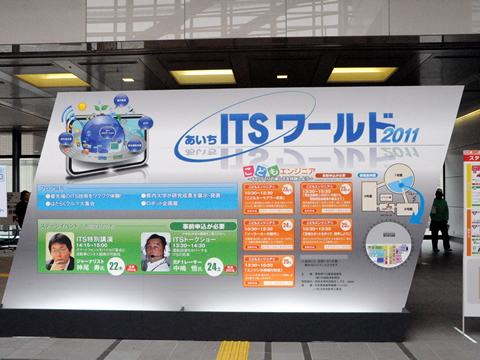
\includegraphics[clip,height=4.0cm]{fig/ITSworld1.jpg}
	\quad
	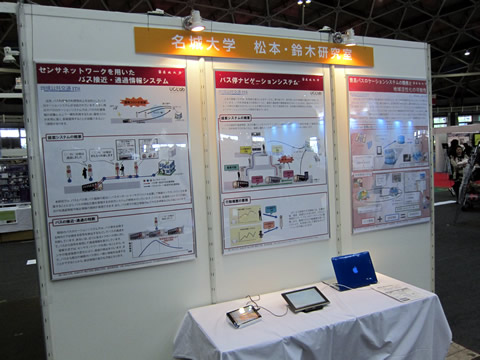
\includegraphics[clip,height=4.0cm]{fig/ITSworld2.jpg}
	\caption{あいちITSワールド2011出展ブースの様子}
	\label{fig:ITSworld}
\end{figure}
\end{enumerate}
% === 展示会(ここまで)=============================

\endinput